%File: formatting-instructions-latex-2024.tex
%release 2024.0
\documentclass[letterpaper]{article} % DO NOT CHANGE THIS
\usepackage{aaai24}  % DO NOT CHANGE THIS
\usepackage{times}  % DO NOT CHANGE THIS
\usepackage{helvet}  % DO NOT CHANGE THIS
\usepackage{courier}  % DO NOT CHANGE THIS
\usepackage[hyphens]{url}  % DO NOT CHANGE THIS
\usepackage{graphicx} % DO NOT CHANGE THIS
\urlstyle{rm} % DO NOT CHANGE THIS
\def\UrlFont{\rm}  % DO NOT CHANGE THIS
\usepackage{natbib}  % DO NOT CHANGE THIS AND DO NOT ADD ANY OPTIONS TO IT
\usepackage{caption} % DO NOT CHANGE THIS AND DO NOT ADD ANY OPTIONS TO IT
\frenchspacing  % DO NOT CHANGE THIS
\setlength{\pdfpagewidth}{8.5in}  % DO NOT CHANGE THIS
\setlength{\pdfpageheight}{11in}  % DO NOT CHANGE THIS
%
% These are recommended to typeset algorithms but not required. See the subsubsection on algorithms. Remove them if you don't have algorithms in your paper.
\usepackage{algorithm}
\usepackage{algorithmic}

%
% These are are recommended to typeset listings but not required. See the subsubsection on listing. Remove this block if you don't have listings in your paper.
\usepackage{newfloat}
\usepackage{listings}
\DeclareCaptionStyle{ruled}{labelfont=normalfont,labelsep=colon,strut=off} % DO NOT CHANGE THIS
\lstset{%
	basicstyle={\footnotesize\ttfamily},% footnotesize acceptable for monospace
	numbers=left,numberstyle=\footnotesize,xleftmargin=2em,% show line numbers, remove this entire line if you don't want the numbers.
	aboveskip=0pt,belowskip=0pt,%
	showstringspaces=false,tabsize=2,breaklines=true}
\floatstyle{ruled}
\newfloat{listing}{tb}{lst}{}
\floatname{listing}{Listing}
%
% Keep the \pdfinfo as shown here. There's no need
% for you to add the /Title and /Author tags.
\pdfinfo{
/TemplateVersion (2024.1)
}


\usepackage{makecell}

% DISALLOWED PACKAGES
% \usepackage{authblk} -- This package is specifically forbidden
% \usepackage{balance} -- This package is specifically forbidden
% \usepackage{color (if used in text)
% \usepackage{CJK} -- This package is specifically forbidden
% \usepackage{float} -- This package is specifically forbidden
% \usepackage{flushend} -- This package is specifically forbidden
% \usepackage{fontenc} -- This package is specifically forbidden
% \usepackage{fullpage} -- This package is specifically forbidden
% \usepackage{geometry} -- This package is specifically forbidden
% \usepackage{grffile} -- This package is specifically forbidden
\usepackage{hyperref} % -- This package is specifically forbidden
%\usepackage{navigator} % -- This package is specifically forbidden
% (or any other package that embeds links such as navigator or hyperref)
% \indentfirst} -- This package is specifically forbidden
% \layout} -- This package is specifically forbidden
% \multicol} -- This package is specifically forbidden
% \nameref} -- This package is specifically forbidden
% \usepackage{savetrees} -- This package is specifically forbidden
% \usepackage{setspace} -- This package is specifically forbidden
% \usepackage{stfloats} -- This package is specifically forbidden
% \usepackage{tabu} -- This package is specifically forbidden
% \usepackage{titlesec} -- This package is specifically forbidden
% \usepackage{tocbibind} -- This package is specifically forbidden
% \usepackage{ulem} -- This package is specifically forbidden
% \usepackage{wrapfig} -- This package is specifically forbidden
% DISALLOWED COMMANDS
\nocopyright % -- Your paper will not be published if you use this command
% \addtolength -- This command may not be used
% \balance -- This command may not be used
% \baselinestretch -- Your paper will not be published if you use this command
% \clearpage -- No page breaks of any kind may be used for the final version of your paper
% \columnsep -- This command may not be used
% \newpage -- No page breaks of any kind may be used for the final version of your paper
% \pagebreak -- No page breaks of any kind may be used for the final version of your paperr
% \pagestyle -- This command may not be used
% \tiny -- This is not an acceptable font size.
% \vspace{- -- No negative value may be used in proximity of a caption, figure, table, section, subsection, subsubsection, or reference
% \vskip{- -- No negative value may be used to alter spacing above or below a caption, figure, table, section, subsection, subsubsection, or reference

\setcounter{secnumdepth}{0} %May be changed to 1 or 2 if section numbers are desired.

% The file aaai24.sty is the style file for AAAI Press
% proceedings, working notes, and technical reports.
%

% Title

% Your title must be in mixed case, not sentence case.
% That means all verbs (including short verbs like be, is, using,and go),
% nouns, adverbs, adjectives should be capitalized, including both words in hyphenated terms, while
% articles, conjunctions, and prepositions are lower case unless they
% directly follow a colon or long dash
\title{Cruciformer: Crossword Clue-to-Answer Transformers}
\author {
    Mike Chaberski
}
\affiliations {
    NYU Tandon School of Engineering\\
    mac937@nyu.edu
}

\begin{document}

\maketitle

\begin{abstract}
    The design, implementation, and evaluation of transformer neural network models for answering crossword puzzle clues is explored herein. Two models are developed: one that considers answers as sequences of words, and another that considers answers as sequences of letters. Hyperparameters are selected by comparing loss curve trends from training. Different methods of generating sequences for answers are devised and compared. Performance of the models is evaluated using a non-neural-network algorithm for answering clues as a baseline. [Comment on performance.] Avenues for further research are suggested in the conclusion.
    Model definition, training, and evaluation code is available at \url{https://github.com/mike10004/csgy6953-fp1}.
\end{abstract}

\begin{NoHyper}

\section{Introduction}
\label{sec:intro}

Determining the answers to crossword puzzle clues involves skills ranging from plundering a mental thesaurus (Recoil from~\textrightarrow~DETEST), to pop culture fluency (Shrek princess~\textrightarrow~FIONA) to clever, lateral reasoning (Swallow things~\textrightarrow~NESTS). Machines are conventionally thought to be good at the more rote skills and less successful at the more abstract ones.

Solving crossword puzzles requires determining the answers to clues, subject to constraints. There are several possible answers to some clues (Historical span~\textrightarrow~AGE/ERA/PERIOD). Constraints such as prior known letters and the answer length reduce the field of possible answers. However, that field is not well-bounded: crossword constructors are free to use arbitrary phrases and neologisms (What's best on the block?~\textrightarrow~PRIME CUTS; Social media-induced anxiety~\textrightarrow~FOMO).

The basis for a good crossword puzzle solving algorithm is a clue solver that can answer the thesaurus clues as well as the abstract ones, while utilizing the additional information from priors such as answer length and known letters.

\section{Related Work}
\label{sec:related}

The intuition behind the use of transformers for answering clues is the robust performance of transformer models at the machine translation task~\cite{vaswani2017}. Mapping crossword clues to answers is a sequence-to-sequence translation task, with the caveats that the source sequences (clues) are generally terse and often contain misdirection, and the target sequences (answers) are generally very short relative to the length of the source sequence.

Crossword solving in general is addressed by~\citealp{kulshreshtha2022across} and~\citealp{wallace2022automated}, both of which efforts implement and evaluate end-to-end algorithms for solving an entire grid. [Describe Berkeley method and Benchmark method.]

The task this study investigates is limited to answering clues, which is a type of reverse-dictionary problem tackled in~\citealp{zhang2019multichannel}. [Describe MultiRD model/results/baseline.] A more fundamental approach to answering clues is implemented in~\citealp{baselinesolver}.
That work does not train a model on a clue-answer database, but instead uses word embeddings to maximize similarity to clues in a database, and selects answers based on best-matching clues.

The concept of answering clues subject to constraints such as word length and known letters is also relevant to this study. Using positional encoding to control output sequence length is a topic addressed by~\citealp{takase2019positional}. The known-letters constraint can be seen as a specific instance of the general problem of unmasking partially-masked sequences given an input context, which is tackled by~\citealp{raffel2023exploring}, among others. Those advanced techniques are not explored herein, though the length constraint is addressed by a text generator algorithm and the performance gain given a known prefix is discussed in the results section.


\section{Dataset}
\label{sec:dataset}

The dataset used by Benchmark is employed in this study on the basis that it is reasonably clean (free of clues for cryptic crosswords, which have categorically different structure and purpose) and pre-segmented in an uncomplicated manner. Segmentation is the breaking up of answer strings into component words, e.g. GETOUT~\textrightarrow~GET~OUT. The segmentation is automated using a dictionary to suggest possible segmentations of a string, and then choosing a result based on likelihood and low word count.

The original Benchmark dataset contains a training set of 433K clue-answer pairs as well as validation and test sets of about 72K pairs each. As discussed below, initial results pointed towards a better path of using a subset of the original set that contains only pairs where the answer is a single word, and removing cross-referential clues (e.g. ``See 46-Across''). This subset is referred to as Onemark and contains 320K pairs in the training set, 55K in the  validation set, and 59K in the test set.

\section{Implementation}
\label{sec:impl}

The two primary parts of the Cruciformer codebase are the model implementation and the answer generation implementation. Model structure and training code was adapted from a transformer implementation for sequence to sequence translation~\cite{chegde2022}. The sequence generator included with that codebase performed only greedy generation, which is not sufficient for analysis of ranked results, so a new sequence generator was implemented with custom parameters to control output sequence length and number of candidate output sequences.

\section{Model Selection}
\label{sec:model}

TODO

\begin{figure}[t]
\centering
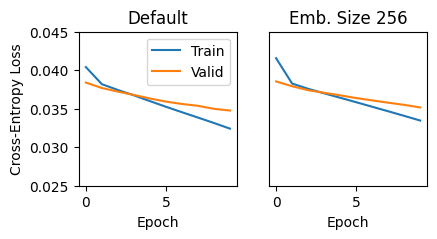
\includegraphics[width=0.9\columnwidth]{fig-onemark-loss-default-and-embsize}
\caption{\textbf{Word model} training and validation loss curves for default hyperparameters and reduced embedding size.}
\label{fig:fig1}
\end{figure}

\begin{figure*}[t]
\centering
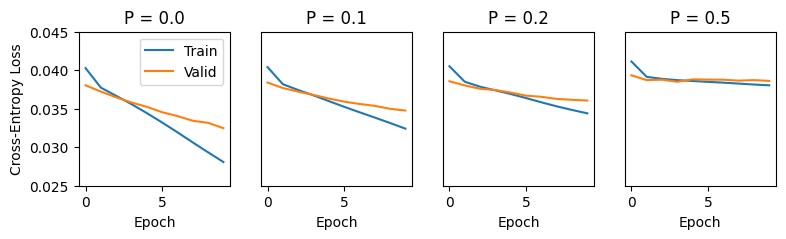
\includegraphics[width=0.8\textwidth]{fig-onemark-loss-dropout}
\caption{\textbf{Word model} training and validation loss curves under varying dropout rates.}
\label{fig:fig2}
\end{figure*}

\subsection{Word Model}
\label{subsec:word}

As shown in~\ref{fig:fig1}, the loss curves are TODO.

\subsection{Letter Model}
\label{subsec:letter}

TODO

\section{Generator Strategy}
\label{sec:generator}

Given a sequence-to-sequence transformer model, a sequence generator is the component that accepts as input a source sequence and an empty or partial output sequence and produces the next element of the output sequence. The generator is iteratively applied to produce a complete sequence. For both the word and letter models, the source sequence is a clue. The word model generator produces a sequence of words and the letter model generator produces a sequence of letters.

For each input, the generator produces an array of values corresponding to possible next tokens. The values are relative measures of likelihood. Our generator implementation applies the softmax function to these values to map them to a probability distribution. (This is the default behavior of the implementation, but other mappings are supported.)

To produce a list of candidate answers for a given clue, beam search is performed. In beam search, the tree of sequence possibilities is traversed and the resulting answers are ranked by their cumulative probability. The cumulative probability of an answer is the product of the probabilities of the constituent sequence elements (words or letters, depending on the model).

At each node of the tree, the possible next tokens are considered in order of probability, descending, up to a limit parameter. We identify a given tree search strategy by the sequence of these limit parameters, so a strategy that looks at the top 10 tokens, then top 5, then top 3, would be identified by the string L10-5-3. For brevity, the last number in the identifying sequence is assumed for all subsequent decision nodes, so a strategy that considers 2 tokens at every node is identified by the string L2. Next tokens are always considered in order of probability.

Different strategies for generating answers are compared below by evaluating their performance in producing correct answers. Because this generator strategy is exponential in runtime by nature, evaluation was performed on a random 1000-pair subset of the validation set. The letter model was evaluated on a subset that contains only answers up to 5 letters in length. Performance is measured by calculating the percentage of correct answers at incremental ranks. For example, the accuracy at rank 10 is the percentage of clue-answer pairs for which the correct answer is among the top 10 candidate answers.

\section{Results}
\label{sec:results}

TODO

\section{Conclusion}
\label{sec:conclusion}

TODO

\bibliography{aaai24}

\end{NoHyper}

\end{document}
